\documentclass[finalversion]{usetex-v1}

%% For intial submission uncomment the following code to remove ednote
%% comments

%\makeatletter{}
%\newsavebox{\kfl@discard}
%\renewenvironment{ednote}[1]{\@latex@warning
%  {Leftover ednote environment in final version ignored}%
%  \begin{lrbox}{\kfl@discard}}{\end{lrbox}}
%\makeatother{}

\usepackage{preamble}

\usepackage{hyperref}
\hypersetup{pdftitle = {mGTK: An \sml binding of \gtk},
            pdfauthor = {Ken Friis Larsen \& Henning Niss},
            pdfsubject = {Describtion of a Standard ML language
              binding for the graphical toolkit \gtk.},
            pdfstartview = {FitH}
            }


% Hacks
\setcounter{secnumdepth}{1}
\newcommand*{\andshare}{\end{tabular}\\\begin{tabular}[t]{c}}



\begin{document}

\title{mGTK: An \sml binding of \gtk}%\\\relax[Extended Abstract]}

\docstatus{Submitted to USENIX'04 (FREENIX track)}

\author{
\authname{Ken Friis Larsen}
\authurl{\url{ken@friislarsen.net}}
\and
\authname{Henning Niss}
\authurl{\url{hniss@it.edu}}
%
\andshare{}
\authaddr{Department of Innovation}
\authaddr{IT University of Copenhagen}
\authaddr{Denmark}
%
} % end author

\maketitle

\DefineShortVerb{\!}

\begin{abstract}
  We describe \mgtk, a Standard ML language binding for the \gtk
  toolkit.  \gtk is a graphical toolkit for the X Window System, and
  provides an object-oriented C language API.  Since Standard~ML is a
  mostly-functional language without object types, constructing a
  binding to \gtk is not a trivial task.  This paper describes
  how it is possible to encode a single-inheritance class-hierarchy
  using \sml's type system. And we describe how we machine-generate
  most of the binding to best utilize the limited man-power of the
  project.  
  
  What we seek to achieve with \mgtk is ``just'' to present a
  type-safe interface to \gtk for \sml programmers.  We are explicitly
  not trying to do, is to figure the best possible way to make an \sml
  graphical user interface, in contrast to what is typically done for
  GUI libraries for functional languages.
%% FIXME
%%   \begin{ednote}{Bart}
%%     You will also want to add a few sentences, describing the
%%   rest of the paper contents, and describing impacts and contributions
%%   of the work.
%%   \end{ednote}

\end{abstract}



\section{Introduction}
\label{sec:intr-backgr}

%This section gives a brief introduction to \sml and \gtk, and presents
%an overview of the rest of the paper.
%
Making a good Standard~ML (\sml) binding to \gtk is an advantage for
both the \sml community and for the \gtk community.  For the \sml
community the two main advantages are: First, \sml programmers get
access to a good general-purpose graphical user interface (GUI)
library with a large range of modern widgets, and the \sml community
is sorely missing such a library.  Second, on a more long term basis, when
we have wrapped the whole GNOME platform, it will be possible for \sml
programmers to make real applications without having to invent add-hoc
solutions to many standard problems, like database access, for
instance.  To the \gtk community the two main advantages of an \sml
binding are: First, that such a binding can help open up the small,
but important, market of teaching languages.  Second, as \sml is a
radically different language than C, an \sml binding will test the
``interfaceability'' of \gtk which is an important design goal for the
\gtk developers.



\subsection{Standard ML}


\sml is a functional language with imperative features which is
widely used for teaching and research.  It is roughly on the same
level of abstraction as Python or Scheme. In contrast to Python and
Scheme, which are \emph{dynamically typed}, \sml is \emph{statically
  typed} (like Java and C++) which means that type errors are detected
at \emph{compile time} rather than at \emph{run time}.  Despite \sml
being statically typed, it is not necessary for the programmer to
explicitly provide type annotations in the program. \sml features
\emph{type inference} which means that the compiler reconstructs type
annotations as needed.

\sml is one of the few languages with a formal definition
\cite{Milner:1997:Definition}.  The definition defines \sml in 93
pages of mathematical notation (a "big step" structured operational
semantics, plus type inference rules) and English prose.  The book is
not meant as tutorial for the language. Rather, it provides an
implementation-independent formulation of \sml.  This formal
definition means that it is possible to write substantial applications
in \sml that are not dependent on a specific compiler.  There are also
several mature \sml implementations with widely different
implementation strategies ranging from byte-code interpreters with
interactive \emph{read--eval--print--loops} (REPLs) to aggressive
whole-program optimizing compilers targeting native code.




\subsection{\gtk}
\label{sec:gtk}


\gtk (The GIMP Toolkit) \cite{Gtk-webpage:2004} is an LGPL-licensed
\cite{LGPL:1999} library for creating graphical
user interfaces.  It works on many UNIX-like platforms, Windows, and
on Linux framebuffer devices.  \gtk is the graphical toolkit used in
the \gnome platform. \gtk is implemented in C with an object-oriented
hierarchy of user interface elements (``widgets''), but from the beginning
the \gtk developers have paid attention to making it feasible and
practical to develop ``bindings'' or ``wrappers'' for
other programming languages than C.  Such bindings allows \gtk to be
used in programs written in those languages. See
\cite{Gtk-bindings-webpage:2004} for a current list of bindings.

The \gtk library itself only contains widgets, but it is built on a
number of useful libraries, to which it is often associated. The main
ones are~\cite{gtk-reference-manual}:
\begin{description}
\item[GLib] A general-purpose utility library, not specific to
  graphical user interfaces. GLib provides many useful data types,
  macros, type conversions, string utilities, file utilities, and so
  on.

\item[Pango] A library for internationalized text handling. It
  provides the rendering engine for the widgets in \gtk that displays
  text.

\item[ATK] The Accessibility Toolkit. It provides a set of generic
  interfaces allowing accessibility technologies to interact with a
  graphical user interface.  \gtk widgets have built-in support for
  accessibility using the ATK framework.

\item[GDK] The abstraction layer that allows GTK+ to support multiple
  windowing systems.
\end{description}
However, in this paper we are concentrating on the widgets only.


%% FIXME
%% \begin{ednote}{Bart}
%%      "It is the graphical toolkit used in the GNOME platform."  Add more
%%    sentences to this to make a paragraph with a brief history of
%%    GIMP/GNOME/Gtk/Gtk+.
%% \end{ednote}

%% \begin{ednote}{Bart}
%%      "...than C."  Should section 4 material move here to
%%    describe the gtk.defs file?
%% \end{ednote}



\subsection{Overview of this paper}
\label{sec:overview-this-paper}

The rest of this paper is organized as follows.
Section~\ref{sec:brief-intr-sml} gives a brief introduction to \sml.
Section~\ref{sec:example} shows a ``Hello World'' example using \mgtk.
Section~\ref{sec:encoding-classes} explains how a single-inheritance
class-hierarchy, in particular \gtk's, can be encoded in \sml's type
system, while retaining type safety.  Section~\ref{sec:process}
describes the work process we have used to make the \mgtk library.
Section~\ref{sec:mgtk-binding} describes practical matters of \mgtk,
such as which \sml compilers are supported.  Finally,
Section~\ref{sec:related-work} lists related work and
Section~\ref{sec:conclusion} concludes.



\section{Brief Introduction to \sml{}}
\label{sec:brief-intr-sml}

This section gives a brief overview of some of the main features of
\sml{}.  It is not enough to use the language to make real programs,
but it should be sufficient to get an understanding of the examples in
the rest of the paper.  We refer the interested reader to one of the
fine textbooks \cite{Hansen-Rischel:1999,Paulson:1996} for more
information about \sml{}.

%% \begin{ednote}{HN}
%% I don't like the sentence ``\ldots use the language in anger'' (what
%% does this ``anger''-thing mean?).
%% \end{ednote}

%% \begin{ednote}{Ken}
%%   It mean something like ``use it for real work''.  See fx 
%%   http://homepages.inf.ed.ac.uk/wadler/papers/sigplan-angry/sigplan-angry.ps
%%   for a good explaination.
%% \end{ednote}

\sml{} is a two-level language, it consists of a \emph{core language}
for programming in the small (that is, functions, data structures and
algorithms), and a \emph{module language} for programming in the large.


\begin{figure*}[thp]
\mbox{}\hfill{}

\begin{subfloat}
\begin{minipage}[b]{.46\linewidth}
\begin{verbatim}
signature STACK = sig 
  type 'a stack
  exception EmptyStack
  val empty : 'a stack
  val push  : 'a * 'a stack -> 'a stack
  val pop   : 'a stack -> 'a * 'a stack
end
\end{verbatim}
\end{minipage}
\caption{\label{fig:stack-sig}interface}
\end{subfloat}
\qquad
\begin{subfloat}
\begin{minipage}[b]{.46\linewidth}
\begin{verbatim}
structure Stack :> STACK =
struct
  datatype 'a stack =
           Empty
         | Stack of 'a * 'a stack
  exception EmptyStack
  val empty = Empty
  fun push(elem, stack) = 
      Stack(elem, stack)
  fun pop stack =
      case stack of
          Empty => raise EmptyStack
        | Stack(top, rest) => 
          (top, rest)
end
\end{verbatim}
\end{minipage}
\caption{\label{fig:stack-struct}implementation}
\end{subfloat}
\hfill\mbox{}
\caption{Simple stack library implemented in SML.}
  \label{fig:stack-lib}
\end{figure*}

Figure~\ref{fig:stack-lib} shows a small stack library implemented in
SML.  This example shows most of the important features of SML.  The
library consists of two parts: an interface description, which is
called a \emph{signature} in SML (Figure~\ref{fig:stack-sig}), and an
implementation module, which is called a \emph{structure} in SML
(Figure~\ref{fig:stack-struct}).  Informally speaking, a
signature is the ``type'' of a structure. It specifies the
declarations of the structure that is to be visible from the outside.


The signature is named !STACK!, its extent is delimited by
\texttt{sig} \ldots\ \texttt{end}, and it contains five
specifications: one type specification, one exception specification,
and three value specifications.

The type specification !type 'a stack! states that a module that
satisfies (implements) the signature !STACK! must declare a type named
!stack! and that this type is parameterized.  The !'a! is a \emph{type
  variable} and this is what makes the type parameterized.  Type
variables can be instantiated to other types.  Thus, the type of a
stack of integers is !int stack!, the type of a stack of integer
stacks is !int stack stack!, and so on. Type variables are at the core of
\emph{parametric polymorphism} (also known as generics in, for
example, C++ and Java; see \cite{garcia03:generics} for a comparison
of programming languages with support for parametric polymorphism).
The type specification does not say anything about how a stack must be
implemented.

The exception specification just states that an exception named
!EmptyStack! must be declared.

The first value specification says that a constant named !empty! must
be declared and that this constant must have type !'a stack!.  That
is, !empty! is a \emph{polymorphic} value, it can be used in contexts
where an \texttt{int stack} is needed or in contexts where a
!int stack stack! is needed.  The next value specification states that a
function named !push! must be implemented, and that this function
takes two arguments: an element and a stack, and returns a stack.
Again, we see how type variables are used to specify that !push! must
work with stacks where the elements can have any type.  The last value
specification states that a function named !pop! must be implemented,
and that !pop!  takes a stack as argument and returns an element and a
new stack.

Figure~\ref{fig:stack-struct} shows the code of the implementation, that is a
structure declaration.  The declarations states
that the structure is named !Stack!, that !Stack! satisfies the
signature !STACK!, and that !Stack! does not reveal any implementation
details not revealed by !STACK! (that is what the !:>! means).  The
extent of a structure is delimited by \texttt{struct} \ldots\ 
\texttt{end}.

The parameterized type !stack! is implemented by an algebraic data
type, that is, the !datatype! declaration.  This declaration says that
an !'a stack! is either: the constant !Empty! or constructed by
applying the constructor !Stack! to an element and a stack (constants
declared by a !datatype! declaration, such as !Empty!  is sometimes
called unit constructors or just constructors).

The exception declaration !exception EmptyStack! just declares an
exception.

The next declaration states that !empty! is bound to !Empty!.  The
function !push! just applies the constructor !Stack! to its arguments.
The function !pop! is more interesting, it takes a stack as argument
(here we have reused the name !stack! as types and values uses
different name spaces, thus the same name can be used for both a type
and a value) and then uses a !case! expression to analyze its argument.
If the argument is the empty stack (the constant !Empty!) then the
exception !EmptyStack! is raised (thrown); otherwise, if the argument
has been constructed with !Stack! applied to the arguments !top! and
!rest! then a pair consisting of !top! and !rest! is returned.

Now, users of this library can call functions from the structure
!Stack! by using ``dot-notation'', for example !Stack.pop mystack!.

This small example illustrate one of the cornerstones in functional
programming, namely that new values are constructed by analyzing,
composing, and sharing old values, in contrast to imperative and
object-oriented programming where values are copied and modified
(although, a new trend in object-oriented programming is to simulate a
functional style, see for example \cite[Item 13 and
14]{bloch01:effective-java}).





%  \sml also features algebraic
%datatypes, pattern-matching, tuples and records, first-class and
%anonymous functions, exception handling, immutable data types and
%updatable references, abstract data types, and parametric modules, but
%it is outside the scope of this paper to introduce all these features,
%instead 





\section{``Hello World'' in \mgtk}
\label{sec:example}

Figure~\ref{fig:hello-world} shows a deliberately simple ``Hello World''
example using \mgtk. It illustrates (1)~how to get the toolkit
initialized using \texttt{GtkBasis.init} (from a module containing
basic \gtk functionality not related to specific widgets), (2)~how to
construct new widgets (using module \texttt{Window} for the Window
widget, and \texttt{Button} for the Button widget), and (3)~how to
connect signals to widgets (using module \texttt{Signal}).

\begin{figure*}[htp]
\begin{centering}
\begin{verbatim}
structure HelloWorld = struct
  fun hello _ = print "Hello World\n"

  fun main _ =
      let val _ = GtkBasis.init(CommandLine.name()::CommandLine.arguments())
          val window = Window.new ()
          val button = Button.new_with_label "Hello World"
      in  Signal.connect window (Widget.delete_event_sig (fn _ => false))
        ; Signal.connect window (Widget.destroy_sig GtkBasis.main_quit)
        ; Signal.connect button (Button.clicked_sig hello)
        ; Container.add window button
        ; Widget.show_all window
        ; GtkBasis.main() 
      end
end

val _ = HelloWorld.main()
\end{verbatim}
\caption{Hello World in \mgtk.\label{fig:hello-world}}
\end{centering}
\end{figure*}

Even from this small example we see some of the main advantages of
\sml combined with \gtk.  First of all, there are no type-annotations
in the program source, still the program is statically type-checked by
the compiler and type errors are found and reported at compile-time
rather than at runtime.  Second, in the figure we use a \sml construct
not explained earlier: the expression !fn _ => false!  denotes an
\emph{anonymous function} that returns !false! regardless of what
argument is given (you can use the \emph{wildcard pattern} !_!
(underscore) if you do not care about the arguments to a function).
Anonymous functions are often really handy for small trivial
callbacks, such as this one.  The construct \texttt{let}~\texttt{val}
\textit{x} \texttt{=} \textit{exp} declares the identifier \textit{x}
to be bound to the value obtained by evaluating the expression
\textit{exp}.  If the only reason for evaluating \textit{exp} is any
potential side effect, one can again use the wildcard pattern.
Expressions evaluated for their side effects only can also be
sequentialized using \texttt{;}.  The value \texttt{()}, the nullary
tuple of type \texttt{unit}, can be used as the return value of purely
side-effecting functions.  Finally, in \sml, the double-colon \texttt{::}
denotes the cons operation on lists.  That is, to add an element $x$
to the beginning of a list $\mathit{xs}$ we write $x \texttt{::}
\mathit{xs}$ (in contrast to C++ where double-colon is the module operator).

%% FIXME
%% \begin{ednote}{Bart}
%%    Explicitly say at some point that "The type of an object in
%%    a programming language is defined by the set of values it
%%    can contain."  This makes the par on base types clearer in
%%    my opinion.
%%
%%    Give examples of building up derived types from base types:
%%    in particular, you need to talk about type definitions
%%    explicitly sometime before section 3.
%% \end{ednote}


%% Example base types are {\tUnit} for the unit value \texttt{()},
%% {\tInt} for integer values, and {\tBool} for boolean values. The type
%% of a list of integers is \tList{\tInt}. The type of a function
%% expecting an integer list argument and returning an integer result is
%% \tArrow{(\tList\tInt)}{\tInt}; the \textit{length} function on lists
%% would have such a type, for example. 

%% Some functions never need to
%% ``inspect'' (sub)parts of supplied arguments values; such functions
%% are called \emph{polymorphic}. For example, the function that just
%% returns it's argument unchanged (the ``identity function'') is
%% polymorphic; so is the function that computes the length of a list. We
%% indicate the parts of the values that are not inspected by using type
%% variables $\alpha, \beta, \ldots$ at the corresponding locations in
%% the type. For example, the type of the identity function is
%% $\tArrow{\alpha}{\alpha}$ telling us that we can apply it to any type of
%% argument, and we get back a value of the same type. The
%% \textit{length} function has type $\tArrow{\tList\alpha}{\tInt}$
%% because, regardless of the type of elements in the list (here denoted
%% $\alpha$), the function can compute the length of the list. Such type
%% variables are \emph{instantiated} to (more) specific types when we
%% apply the polymorphic function. For example, when we apply the
%% polymorphic identity function to \texttt{()} we instantiate $\alpha$
%% to {\tUnit} giving this occurrence of the function the type
%% \tArrow\tUnit\tUnit; when we apply it to \texttt{17} we instantiate
%% $\alpha$ to {\tInt} and the occurrence of the function gets type
%% \tArrow\tInt\tInt. The function is said to be (parametric) polymorphic
%% because we can apply it to arguments of many shapes.

%% Some functions never need to
%% ``inspect'' (sub)parts of supplied arguments values; such functions
%% are called \emph{parametric polymorphic}. For example, the 
%% function \textit{length} that computes the length of a list is polymorphic. We
%% indicate the parts of the values that are not inspected by using type
%% variables $\alpha, \beta, \ldots$ at the corresponding locations in
%% the type. Then the type of \textit{length} is
%%  $\tArrow{\tList\alpha}{\tInt}$
%% because, regardless of the type of elements in the list (here denoted
%% by $\alpha$), the function can compute the length of the list. Such type
%% variables are \emph{instantiated} to (more) specific types when we
%% apply the polymorphic function. For \textit{length}, when we
%% apply it to a list of booleans we instantiate $\alpha$
%% to {\tBool} giving this occurrence of the function the type
%% \tArrow{\tList\tBool}\tInt; when we apply it to a list of
%% integers  we similarly instantiate
%% $\alpha$ to {\tInt}.

\section{Encoding of Classes}
\label{sec:encoding-classes}

As described in Section~\ref{sec:intr-backgr}, \sml is a functional
language without object-oriented features and \gtk is designed as an
object-oriented library.  Thus, it is not easy to see how to make an \sml
interface to \gtk.  The most difficult problem is how to present the
subtype relations defined by a class hierarchy in \sml's type system.
That is, in this section we are only interested in how to present a
type-safe \sml interface to the \gtk class hierarchy.  By \emph{type-safe} we
mean that, if an \sml application programmer uses our library and
makes a type-error when using the \gtk library, calling a undefined
method on object, for instance, then the \sml compiler should give a
type error (at compile-time).

Throughout we shall think of class-hierarchies mainly as definitions
of subtype relationship.  This ``confusion'' of classes and types is
intentional, as this is the right level of abstraction for the paper.

Fortunately, we are able to take advantage of two properties of \gtk
and \sml.  First, \gtk implements a class system with only
single-inheritance.  Second, \sml's type system is expressive enough
to express the subtype relations of single-inheritance class
hierarchies.  Thus, we present a general method of taking a given
object oriented class hierarchy and encoding and encoding it in \sml
type system.  The properties of the resulting encoding are that: each
class type has a corresponding \sml type; the encoding is
\emph{complete}, meaning that all that is allowed by the class
hierarchy is also allowed by the encoding; and the encoding is
\emph{sound}, meaning that all that is disallowed by the class
hierarchy is also disallowed by the encoding.  The last property is
also called type-safety.  In type-theoretical jargon, the trick is to
use parametric polymorphism and \emph{existential types} to encode
inheritance subtyping.  In particular we use \emph{phantom types} to
encode the inheritance path.


\begin{figure}[htp]
  \centering
% 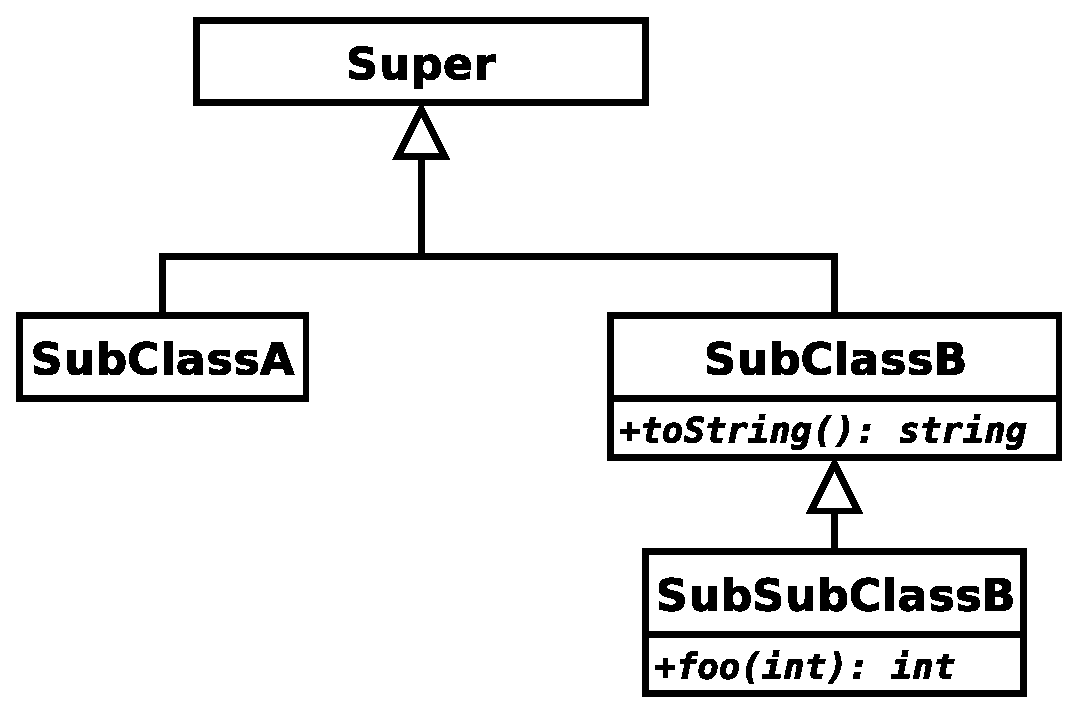
\includegraphics[width=.8\linewidth]{example-class-diagram.eps}
%  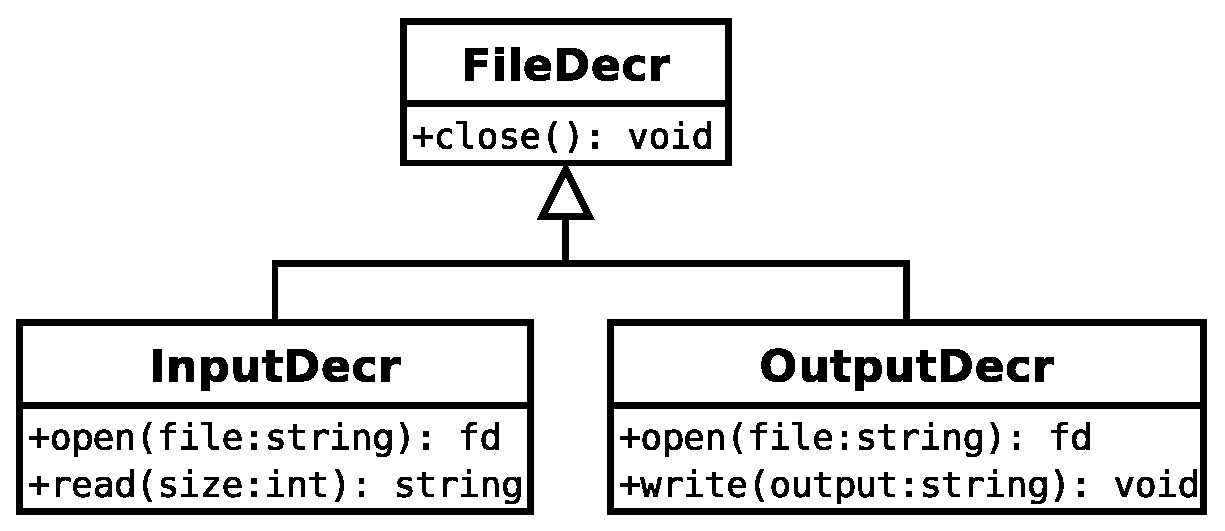
\includegraphics[width=.8\linewidth]{filedecr-class-diagram.eps}
  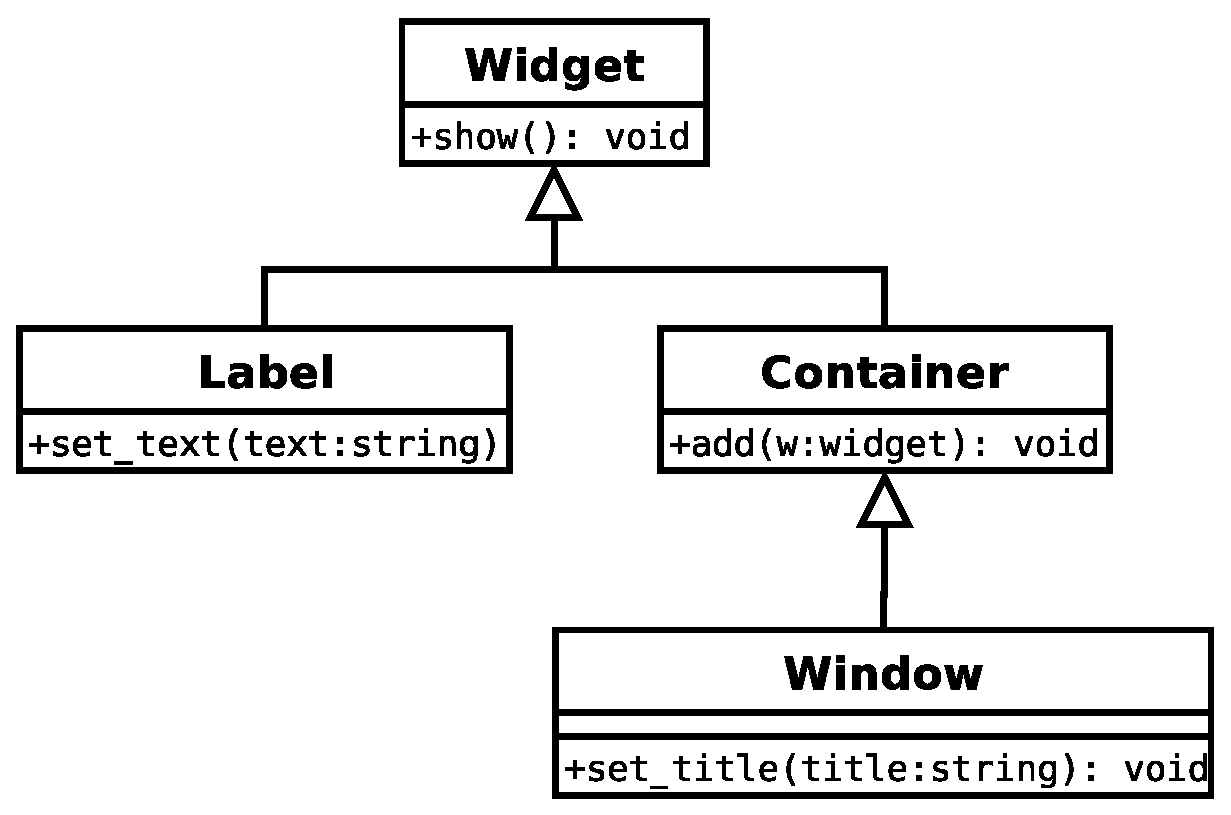
\includegraphics[width=.9\linewidth]{widget-class-diagram.mps}
  \caption{Small example class hierarchy}
  \label{fig:class-hierarchy}
\end{figure}

Figure~\ref{fig:class-hierarchy} shows a small class hierarchy with
just four classes. \classname{Label} and \classname{Container} are
subclasses of the class \classname{Widget} and \classname{Window} is a
subclass of \classname{Container}.  For the specific class hierarchy
in Figure~\ref{fig:class-hierarchy}, the properties we want to enforce
with our type encoding into \sml's type system are: that we should be
allowed to call the !show! method on all kinds of arguments whether
they are of class type \classname{Widget}, \classname{Label},
\classname{Container}, or \classname{Window}; that we should be
allowed to call the !add! method on \classname{Container}s and
\classname{Window}s, but not \classname{Widget}s and
\classname{Label}s; that we should only be allowed to call !set_title!
on \classname{Window}s; and so on.

We now go through the different parts of the encoding of a class.
Throughout this description we only present the \sml specifications.
That is, the parts that go into the signatures. The parts that go into
the structures is not as interesting as that is simply a matter of
calling into the C runtime.

\begin{description}
\item[Class types] A base class like \classname{Widget} in
  Figure~\ref{fig:class-hierarchy} is encoded as an abstract
  parameterized type:
\begin{SMLcode}
type 'path widget
\end{SMLcode}
(we follow the convention suggested by the \smlbasis and spell
type-names in lower-case with underscores if needed).  The type
variable !'path! will be used to hold the inheritance path for
subclasses.


\item[Subtyping/Inheritance] For a subclass like \classname{Label} we
  need to encode two things: that the class (type) exists and the
  subtype relation to the parent class.  To do this, we declare two
  new \sml types: an abstract parameterized type; and a type
  abbreviation for specifying the inheritance:
\begin{SMLcode}
type 'path label_t
type 'path label = 
        'path label_t widget
\end{SMLcode}
We call the abstract type (here !label_t!) the \emph{witness type}
because it witness that the class exists.  Similar, the type !label!
is the type abbreviation that specifies that \classname{Label} inherits
from \classname{Widget}.  In the declaration of !label!  we see that
the type variable !'path! in the declaration of the type !widget!  has
been instantiated with the type expression !'path label_t!, which
contains a new type variable (also named !'path!).

In the rest of the paper we shall use the convention that witness
types ends with !_t!.

This is the juicy bits of the encoding, because this is really what
makes it possible to encode single-inheritance class hierarchies in
\sml.  Unfortunately, this is also the hardest part of the encoding to
understand.  Our experience is that you have to work a bit with some
code to really comprehend the trick.


%% \begin{ednote}{Bart}
%%   Note in particular that typing the running example into ML will
%%   result in an error, since type specifications are available only in
%%   signatures.  This is a bit confusing to even a knowledgeable reader
%%   (e.g. me :-).
%% \end{ednote}

\item[Methods] Because \sml is not an object-oriented language we shall
  model methods with ordinary functions and use the usual convention
  that the first argument is the object on which the method is called.
  (\gtk also uses this convention).
  
  We can now write the type for the method !add! in
  \classname{Container}:
\begin{SMLcode}
val add : 'path container -> 'a widget 
                               -> unit
\end{SMLcode}
This type says that !add! takes two arguments: an object of type
\classname{Container} and a widget, and returns !unit! as result.
Similar the type for the method !set_title! from class
\classname{Window} has the type:
\begin{SMLcode}
val set_title : 'path window -> string 
                               -> unit
\end{SMLcode}
That is, !set_title! takes two arguments: an object of type 
\classname{Window} and a string, and returns !unit!.


\item[Constructors] We have to be a bit careful with constructors.  If
  we were to return a value with a polymorphic type-variable !'path!
  that holds an inheritance path that has not yet been ``plugged'',
  then we can accidentally use a super-class constructor to construct
  values that can be instantiated to the type of a sub-class.  Hence,
  we introduce the abstract dummy type !base! and use that to plug the
  type variable.  Thus, the type of the constructor for
  \classname{Label} is:
\begin{SMLcode}
type base
val new : unit -> base label
\end{SMLcode}
The convention in \gtk is that constructors are named !new!.

\item[Fields] We are not able to handle fields directly, because we
  keep the representation of objects completely opaque.  Thus, all
  inspections and changes to fields must be done though getter and
  setter methods.

\end{description}

We then wrap all parts of an encoding of a class into a signature,
structure pair of its own.  That is, for the class \classname{Window}
in Figure~\ref{fig:class-hierarchy} the \sml signatures is:
\begin{SMLcode}
signature Window =
sig
  type 'path window_t
  type 'path window = 
      'path window_t Container.container
  val new : unit -> GtkBasis.base window
  val set_title : 'path window -> string 
                                 -> unit
end
\end{SMLcode}
We see that this signature relies on two structures: The structure
!Container! for the class \classname{Container} and !GtkBasis! for the dummy
type !base!.  In addition to the signature !Window! we also need a
structure called !Window! that implements the actual calling of the
relevant \gtk C functions.

Now, does this encoding really allow all the things that the class
hierarchy allows?  Yes, for example, the function
\texttt{Container.add} has type:
\begin{SMLcode}
val add : 'p1 container -> 'p2 widget 
                                 -> unit
\end{SMLcode}
From this type we can see that, if !label! is a value of type 
%
!base label! 
% 
and !window! is a value of type !base window! then
the application
%
!Container.add window label!
%
is well-typed because: (1)~the type of !window! is just a abbreviation for 
%
!base window_t container!,
%
thus, the type variable !'p1! can be instantiated to 
%
!base window_t!,
% 
and (2)~the type of !label! is just an abbreviation of 
%
!base label_t widget!,
%
thus, the type variable !'p2! can be instantiated to 
%
!base label_t!.

Consider now the function !set_title! that only works on \classname{Window}s:
\begin{SMLcode}
val set_title : 'p window -> string -> unit
\end{SMLcode}
If we, by mistake, attempt to use this function to set the text of the
label !label! (with type !base label!) as in expression
%
!Window.set_title label "New text"!, 
%
we get a (compile-time) type error saying (essentially) that a
\classname{Label} widget is not a subclass of a \classname{Window}
widget because the inheritance paths do not match.  Here is the
concrete error message given by the Moscow ML compiler:
\begin{verbatim}
- Window.set_title label "New text";
! Toplevel input:
! Window.set_title label "New text";
!                  ^^^^^
! Type clash: expression of type
!   base label_t widget
! cannot have type
!   'a window_t container_t widget
\end{verbatim}

Hence, we have demonstrated that our encoding (in these concrete
examples) is both sound and complete.

%% \begin{ednote}{Ken}
%%   Explain the cool signal thing.
%%   (drop for extended abstract)
%% \end{ednote}

%% \begin{ednote}{Ken}
%%   How about the implementation of the binding with finalizers and all?
%% \end{ednote}


\section{Process}
\label{sec:process}

In constructing the \mgtk binding we leverage the foresightedness of
the \gtk developers. Early on it was recognized that it would be
important to have a machine-readable ``specification'' of the toolkit.
Essentially the specification would specify the widget classes, the
inheritance hierarchy, and methods and functions in the toolkit. The
specification became known as the \texttt{gtk.defs} file. One could
argue that it is simple enough to extract the same information from
the C header files. However, C headers are difficult to parse, whereas
the defs format is straightforward to parse.

The bulk of the \mgtk binding is constructed automatically from the
\texttt{gtk.defs} file.  The complete binding process is naturally
divided in two phases: (1) binding ``design'' where we apply the
principles described in Section~\ref{sec:encoding-classes} on a few
representative widgets to demonstrate the structure of the binding,
and (2) binding construction where the structure in (1) is applied to
the entire toolkit. It is important to note here that the design phase
can be carried out for a very small subset of the toolkit after which
the construction phase ``mimics'' that for the complete toolkit.
% We refer to the design as a
%\emph{muck-up} and the result as \minimgtk.
This phase separation makes it easier to get the design right simply
because there are fewer issues to deal with.  It also makes the work
involved in moving the binding to other \sml compilers manageable
(essentially just ask the compiler writers to provide the equivalent
of the small subset for their compiler; and mimic that during the
construction phase). Finally, we hope it will help when new releases
of \gtk are produced. Most of the work in constructing the binding for
the new release is over when the design of the small subset has been
completed.

Let us return to our running example, and look at some example
specifications of widgets, functions/methods, and signals.
Figure~\ref{fig:gtk-defs} shows three entries in the \texttt{gtk.defs}
file.
\begin{figure}[htbp]
\begin{centering}
\begin{verbatim}
(define-object Container
  (in-module "Gtk")
  (parent "GtkWidget")
  (c-name "GtkContainer")
  (gtype-id "GTK_TYPE_CONTAINER")
)

(define-method gtk_container_add
  (of-object "GtkContainer")
  (c-name "gtk_container_add")
  (return-type "none")
  (parameters
    '("GtkWidget*" "widget")
  )
)

(define-signal delete-event
  (of-object "GtkWidget")
  (return-type "gboolean")
  (when "last")
  (parameters
    '("GdkEventAny*" "p0")
  )
)
\end{verbatim}
\caption{\texttt{gtk.defs} excerpt.\label{fig:gtk-defs}}
\end{centering}
\end{figure}
The first entry shows a widget specification indicated by
!define-object!. From the entry we see that the !GtkContainer! widget
(the name appearing right after !define-object! is a shorthand)
inherits from !GtkWidget!, and it belongs in the !Gtk! module.  We also
see the type assigned to instances of this widget in the \emph{\gtk type
system} (which is completely unrelated to the \sml encoding given
above).

The next entry shows a method specification for the method !add!
which does takes a !GtkWidget*! (in the C implementation)
argument, and returns nothing. Since it is a method, there is an
implicit ``self'' argument of type !GtkContainer*!.

The final entry shows a ``signal handler'' or (``callback'')
specification. In this case, we specify the prototype for handlers of
delete events on widgets. The signal handler for !delete-event! for
widget !GtkWidgets! accepts a parameter of type !GdkEventAny*!, and
returns a value of type !gboolean!. 

%\subsection{Stubs and code generation}
%\label{sec:stubs-code-gener}


%% \section{Synergy}
%% \label{sec:synergy}

%% \begin{ednote}{Henning}
%%   SML + Gtk+ er godt
%%   (drop for extended abstract?)
%% \end{ednote}



%% \section{Supported \sml compilers}
%% \label{sec:supp-sml-comp}

%% \begin{ednote}{Henning}
%%   MLton og Moscow ML (SML.NET med Gtk\#?)
%% \end{ednote}

\section{The \mgtk Binding}
\label{sec:mgtk-binding}

The \mgtk binding is available at SourceForge \texttt{http://mgtk.sf.net/}
and is released under the GNU Lesser General Public License
(LGPL) \cite{LGPL:1999}.

A fundamental difference in producing \sml bindings of \gtk compared
to bindings for other languages is the existence of a variety of
compilers (see the reason in Section~\ref{sec:intr-backgr}). This sets
this work apart from bindings to languages such as Python where
there is only one compiler/system to target. 

The encoding of the \gtk class hierarchy in the \sml type system in
Section~\ref{sec:encoding-classes} is \emph{the} core aspect of the
binding. As the encoding stays within the language as defined in the
Definition~\cite{Milner:1997:Definition}, this aspect of the binding
remains the same for all \sml compilers conforming to the Definition.
In other words, the interface exposed to the application programmer is
the same across all compilers.
%
One finds \sml and \gtk implementations on a large variety of
platforms. Thus, the porting work in moving application programs from one of these
platforms to another is non-existent.

The \mgtk binding already targets two of the main \sml systems,
\mosml~\cite{Mosml-webpage:2003} and \mlton~\cite{MLton-webpage:2003}.
The authors are currently looking into the prospects of constructing
the binding for other \sml compilers (in particular, the \emph{ML Kit
  with Regions} \cite{MLKit-webpage:2003} and \emph{SML.NET}
\cite{SML.NET-webpage:2003} with \gtksharp). As mentioned above,
Section~\ref{sec:process}, this is mainly an issue about interfacing
to C.

This potential for compiler independence sets the present binding
apart from other \gtk bindings for \sml; notably, the \texttt{SML-Gtk}
binding for the \sml of New Jersey compiler;
\cite{SML-Gtk-webpage:2003}.  The \texttt{SML-Gtk} binding is also based
phantom types. Our binding predates the \texttt{SML-Gtk} binding with
approximately two years, and the \texttt{SML-Gtk} User's Manual refers to the
\mgtk binding.  To date no serious attempts has been made to join
these two projects.  The reason for this is that even though
the projects seems similar we have followed rather different
strategies for making our respective bindings.  \texttt{SML-Gtk}
partly generated by !ml-nlffi!, for instance, and does not attempt to
automate memory management.

%% \begin{ednote}{Bart}
%%   This work vs SML/NJ?  Is this a replacement for Leung's
%% system?  You need to cite [10] much earlier in the paper,
%% and make it clear that you are not the only ones to use
%% phantom types for this task.  In particular, I don't see how
%% the claim that "the encoding of a single inheritance
%% hierarchy as above is [new]." can be true, given that [10]
%% appears to have a very similar system.  Do you predate this
%% work?

%% \end{ednote}


\section{Related Work}
\label{sec:related-work}

The list of language bindings for \gtk shows a plethora of different
languages from which \gtk is accessible. In this section we briefly
discuss the bindings most related to \mgtk.

When considering ML-like languages, there are two major alternatives
to the \mgtk binding. (1) The !SML-Gtk! binding mentioned above.  This
binding is different from \mgtk in that it is made with the !ml-nlffi!
bindings generator \cite{Blume:2001:nlffi}, which is currently
specific to the SML/NJ compiler.  Furthermore, it does not address
memory management issues.
%
(2) !lablgtk! is a \gtk binding for O'Caml.
O'Caml is a ML dialect different from \sml which (among other things)
has object-oriented features. This binding, therefore, does not have
to \emph{encode} the \gtk object hierarchy.

\gtk has also been bound to other functional languages;
!gtk+hs! is a Haskell binding for example,
% \url{http://www.cse.unsw.edu.au/~chak/haskell/gtk}
and !erlgtk! is an Erlang binding.
% \url{http://erlgtk.sourceforge.net}
%
Also bindings for other graphical toolkits, such as Tk, exists.
For example, !sml_tk! is an \sml binding of Tk.
% \url{http://www.informatik.uni-bremen.de/~cxl/sml_tk}

The use of phantom types to express invariants about the program
is not new; the encoding of a single-inheritance hierarchy as
above is. Independent work has established similar results
\cite{Fluet-Pucella:2002}. %
On the construction side of things, other bindings are also machine
generated; for this some of the bindings use the \emph{Simplified
  Wrapper and Interface Generator} (SWIG) \cite{Beazley:1996}, others
extract appropriate information directly from the C headers files of
\gtk.

From the outset the necessity of access to libraries has been realized
in the functional programming community. Work in this area for \sml
include 
%\mosml's C-library support \cite{Larsen:2001} and 
\smlnj's foreign function interface \cite{Blume:2001:nlffi};
for Haskell it includes \cite{Finne:1999:CallingHellFromHeaven}.



\section{Conclusion}
\label{sec:conclusion}

It is our intention to continue this work by utilizing appropriate
programming language technology to gradually bind more and more of the
\gnome development platform for \sml. As was the case above, this
entails designing appropriate representations of the platform in the
\sml world (in particular as regards the type-safety property mentioned
above) together with the more practical work of extending the code
generator to handle such newly introduced representations.

The long term goal for \mgtk is to target most of the \gnome{}
platform.  The advantages of bringing \gnome to the \sml community in
the form of such bindings would be twofold: firstly, it would allow \sml
programmers access to the vast collection of useful application-level
support in \gnome, and secondly, allow \sml programmers to take part in
the development of \gnome components by allowing them to write such
components in \sml. The key technical aspect to be solved here is to
support type safe inheritance on the \sml side of things. Of course,
one will also have to explore exactly how to tie the various languages
together, but the \gnome community already has experience in this area.

%% \begin{ednote}{Bart}
%%   Expand the discussion here substantially: it sounds
%% interesting.  What will it take to write SML-GNOME apps?
%% What parts will you replicate/replace?  What parts will you
%% just interface to?

%% \end{ednote}

In this paper we have demonstrated that it is theoretically and
practically possible to make a type safe interface from \sml to \gtk.
This is interesting for several reasons: first, \mgtk was one of the
first graphical toolkits available to the \sml community; second, the
fact that it is possible to make an \sml binding to \gtk really
attests to the claimed ``interfaceability'' of \gtk because \sml is so
radically different from C in abstraction level and paradigm; third,
by auto-generating the binding we get a binding of the complete \gtk
toolkit; finally, we believe that the particular way we construct the
binding, gives us hope that we may eventually be able to bind the
entire \gnome development platform, using mainly machine generated
stub code.

\bibliographystyle{abbrvnat}
\bibliography{mgtk}

\end{document}

%%% Local Variables: 
%%% mode: latex
%%% TeX-master: t
%%% TeX-command-default: "PDFLaTeX"
%%% End: 

% LocalWords:  mGTK FREENIX Friis Niss GtkBasis fn wildcard tl gtk defs SML API
% LocalWords:  GtkWidget MLton mgtk interfaceability eval REPLs LGPL GLib Pango
% LocalWords:  framebuffer ATK GDK sig EmptyStack struct datatype mystack init
% LocalWords:  nullary xs subtyping GtkContainer GtkWidgets GdkEventAny nlffi
% LocalWords:  gboolean SourceForge lablgtk O'Caml hs erlgtk Tk sml tk
